\section{Differential Evolution}
\label{sec:de}

Differential evolution (DE)~\ref{storn1997differential} is a population based search heuristic designed to iteratively improve candidate soltions to a problem. DE is best suited for problems containing a nonlinear and non-differentialable continuous search space. DE works by creating a new candidate solution using existing candidate solutions in the population using a \textit{mutation} operator. Once a new candidate solution is creating the fitness scores of each solution are compared and the candidate with the better fitness score is put into the new population. Figure~\ref{fig:deFlowchart} depicts how evolution occurs in DE and Subsections~\ref{subsec:de-mutation} and~\ref{subsec:de-selection} describe the operators used.

\begin{figure}[H]
  \centering
  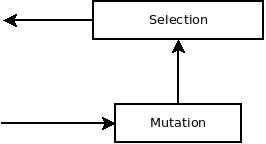
\includegraphics[bb=0 0 266 144,scale=0.5]{figures/DE.jpeg}
  \caption{DE Evolution}
  \label{fig:deFlowchart}
\end{figure}

\subsection{Mutation}
\label{subsec:de-mutation}

\subsection{Selection}
\label{subsec:de-selection}